\section{Resultados}

\subsection{Coleta e qualidade estrutural da base}

A Tabela~\ref{tab:coleta-v2} resume a primeira execução congelada utilizada neste artigo. Os números mostram que a descoberta em escala nacional é viável, mas a extração automatizada ainda é sensível à heterogeneidade operacional das instâncias do SAPL.

\begin{table}[H]
\centering
\caption{Cobertura da coleta na execução congelada de 12/11/2025.}
\label{tab:coleta-v2}
\small
\begin{tabular}{l r r}
\toprule
Métrica & Contagem & Cobertura \\
\midrule
Instâncias SAPL encontradas & 1.259 & 22,60\% dos municípios \\
Instâncias com extração válida & 322 & 5,78\% dos municípios \\
PLs coletados & 220.065 & -- \\
\bottomrule
\end{tabular}
\end{table}

A Tabela~\ref{tab:regioes-v2} detalha a distribuição regional dos registros efetivamente presentes no dataset final. Os resultados evidenciam forte concentração no Sul e no Sudeste, tanto em número de registros quanto em número de municípios representados.

\begin{table}[H]
\centering
\caption{Distribuição regional do dataset final.}
\label{tab:regioes-v2}
\small
\begin{tabular}{l r r}
\toprule
Região & Registros & Municípios \\
\midrule
Sul & 100.175 & 107 \\
Sudeste & 50.673 & 100 \\
Centro-Oeste & 38.788 & 68 \\
Nordeste & 21.588 & 36 \\
Norte & 8.841 & 11 \\
\bottomrule
\end{tabular}
\end{table}

\begin{figure}[H]
\centering
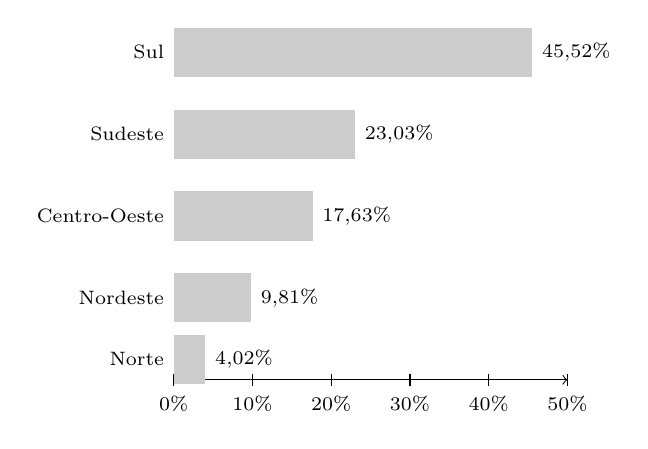
\begin{tikzpicture}[x=0.10cm,y=0.52cm,font=\scriptsize]
\draw[->] (0,0) -- (50,0);
\foreach \x in {0,10,20,30,40,50} {
  \draw (\x,0.15) -- (\x,-0.15);
  \node[below] at (\x,-0.15) {\x\%};
}
\node[left] at (0,8) {Sul};
\fill[black!20] (0,7.4) rectangle (45.52,8.6);
\node[right] at (45.52,8) {45,52\%};
\node[left] at (0,6) {Sudeste};
\fill[black!20] (0,5.4) rectangle (23.03,6.6);
\node[right] at (23.03,6) {23,03\%};
\node[left] at (0,4) {Centro-Oeste};
\fill[black!20] (0,3.4) rectangle (17.63,4.6);
\node[right] at (17.63,4) {17,63\%};
\node[left] at (0,2) {Nordeste};
\fill[black!20] (0,1.4) rectangle (9.81,2.6);
\node[right] at (9.81,2) {9,81\%};
\node[left] at (0,0.5) {Norte};
\fill[black!20] (0,-0.1) rectangle (4.02,1.1);
\node[right] at (4.02,0.5) {4,02\%};
\end{tikzpicture}
\caption{Participação percentual das regiões no total de registros do dataset.}
\label{fig:regioes-v2}
\end{figure}

Em termos percentuais, o Sul concentra 45,52\% dos registros e o Sudeste 23,03\%. Juntas, essas duas regiões somam 68,55\% de todo o acervo. Do ponto de vista municipal, Sul e Sudeste concentram 64,29\% dos 322 municípios presentes na base final.

Do ponto de vista temporal, a base cobre principalmente o período moderno da produção legislativa municipal, mas também contém histórico mais antigo. A data mínima observada foi 29/12/1947. Ao mesmo tempo, a análise exploratória revelou poucos, porém importantes, outliers temporais, incluindo um registro com ano 199 e duas datas de apresentação em 2099. Esses casos sugerem a necessidade de saneamento temporal antes de análises mais sensíveis ao eixo cronológico.

Apesar desses outliers, a massa recente da base é expressiva: entre 2021 e 2025, há 96.018 registros, correspondentes a 43,63\% do dataset, distribuídos por 315 municípios. Esse resultado é relevante para o uso aplicado do sistema, pois mostra que a base não é apenas histórica, mas também suficientemente recente para apoiar consultas contemporâneas.

\subsection{Tradução de ementas em ações}

Na avaliação interna do projeto, o tradutor \textit{ementa} $\rightarrow$ \textit{ação} obteve BERTScore de 84\% no conjunto de validação. Além disso, a transformação de todo o acervo de 220.065 PLs em recomendações de ação levou 4h47min na execução reportada. Esse resultado sugere viabilidade operacional do pipeline, embora ainda faltem comparações com \textit{baselines} adicionais e avaliação humana formal.

A análise exploratória do dataset também mostrou que a textualização reduz substancialmente o comprimento médio das descrições legislativas, sem colapsar a diversidade do acervo. Foram observadas 219.245 ementas únicas e 188.254 ações únicas. Em outras palavras, a tradução não apenas encurta o texto, mas reduz variabilidade superficial o suficiente para favorecer recuperação semântica e agrupamento.

\subsection{Busca semântica}

A etapa de busca semântica foi validada de forma exploratória com consultas reais e julgamento manual de relevância das ações retornadas. Essa análise indicou utilidade prática para o cenário de uso, mas ainda não constitui uma avaliação formal de recuperação da informação. Em especial, ainda não há conjunto anotado de consultas nem métricas consolidadas de ranking. Portanto, os resultados atuais da busca devem ser interpretados como evidência preliminar de utilidade, e não como benchmark conclusivo.

Mesmo sem benchmark formal, a busca já produz saídas plausíveis para consultas substantivas. Para a consulta ``como enfrentar a violência contra a mulher no município?'', a recuperação semântica retornou, entre os cinco primeiros itens, ações como: regulamentar a violência contra a mulher no município (Uruguaiana/RS), criar política municipal de enfrentamento à violência política contra a mulher (Parauapebas/PA e Santo Antônio do Sudoeste/PR), criar programa de práticas de enfrentamento à violência contra a mulher com monitoramento de segurança (Rio Negro/PR) e promover campanha de denúncia da violência contra a mulher (Anápolis/GO). Esse exemplo não substitui avaliação quantitativa, mas mostra que o sistema já retorna recomendações tematicamente alinhadas ao problema informado pelo usuário.

\subsection{Agrupamento de políticas públicas}

A etapa de agrupamento mostrou-se útil para converter recomendações isoladas em políticas recorrentes comparáveis entre municípios. Com limiar de Jaccard fixado em 0,75 e escore heurístico $Q = \frac{n_{\text{positivos}}}{n}\times\frac{n}{n+1}$, foi possível identificar grupos com recorrência temática e evidência observacional suficiente para inspeção qualitativa.

A Tabela~\ref{tab:clusters-v2} mostra três clusters ilustrativos extraídos do recorte temático de violência contra a mulher. Os dois primeiros pertencem à frente de segurança e proteção social; o terceiro representa a frente educacional e preventiva. Em conjunto, eles mostram que o agrupamento consegue reunir proposições semanticamente próximas mesmo quando há variação lexical entre municípios.

\begin{table*}[t]
\centering
\caption{Clusters ilustrativos extraídos com Jaccard = 0,75.}
\label{tab:clusters-v2}
\small
\begin{tabular}{p{0.18\linewidth} p{0.43\linewidth} p{0.10\linewidth} p{0.09\linewidth} p{0.14\linewidth}}
\toprule
Frente & Política representativa & $n$ & $Q$ & Municípios exemplo \\
\midrule
Segurança/proteção & Criar mecanismo de punição administrativa para combater a violência contra a mulher no município. & 3 & 0,750 & Coronel Fabriciano, Cabo de Santo Agostinho, Natal \\
Segurança/proteção & Criar programa municipal de enfrentamento ao feminicídio. & 3 & 0,750 & Armação dos Búzios, Campinas, Olinda \\
Educação/prevenção & Tornar obrigatória o ensino de noções básicas sobre a Lei Maria da Penha nas escolas públicas municipais. & 8 & 0,667 & Campinas, Araxá, Araguari, Rio Grande, Natal \\
\bottomrule
\end{tabular}
\end{table*}

\subsection{Estudo de caso: violência contra a mulher}

Entre os temas disponíveis no acervo, violência contra a mulher foi selecionado como estudo de caso principal desta versão. O recorte lexical correspondente reúne 2.306 ações distribuídas por 204 municípios e 18 UFs. Isso indica que o tema já aparece com massa crítica suficiente para ilustrar o fluxo completo do sistema, desde a consulta em linguagem natural até a consolidação de políticas recorrentes.

No recorte temático com janela de 6 meses para taxa de homicídios, 1.240 ações tiveram efeito computável e geraram 136 políticas agrupadas com pelo menos dois municípios. O cluster com maior escore heurístico foi ``Conceder auxílio financeiro a mulheres vítimas de violência doméstica no município'', com $Q=0,778$, oito municípios representados e sete efeitos favoráveis em oito observações. Entre os exemplos que compõem esse grupo estão Marabá, Campina Grande e Campinas, com reduções observadas de -26,23\%, -22,22\% e -30,00\%, respectivamente.

Além do cluster líder, o estudo de caso mostra diversidade de estratégias substantivas. Entre os agrupamentos com $Q=0,750$, apareceram propostas de tramitação prioritária para processos envolvendo vítimas de violência doméstica, programas de defesa pessoal para mulheres, programas municipais de enfrentamento ao feminicídio e mecanismos de punição administrativa para autores de violência contra a mulher. Em outras palavras, o sistema não concentra as recomendações em uma única família de resposta, mas recupera intervenções de proteção institucional, prevenção e suporte social.

A Tabela~\ref{tab:falhas-v2} resume três falhas concretas observadas durante a inspeção qualitativa. Esses exemplos são importantes porque mostram que os maiores riscos atuais do sistema não estão apenas em cobertura, mas também em condensação textual, limpeza temporal e interpretação ingênua de variações extremas do indicador.

\begin{table}[H]
\centering
\caption{Falhas observadas na inspeção qualitativa do pipeline.}
\label{tab:falhas-v2}
\small
\begin{tabular}{p{0.18\linewidth} p{0.28\linewidth} p{0.42\linewidth}}
\toprule
Etapa & Exemplo & Implicação \\
\midrule
Tradução & ``Junho Violeta'' $\rightarrow$ ``Junho Violento'' & A condensação pode alterar o sentido material da proposta quando o modelo força uma paráfrase inadequada. \\
Base temporal & Registros com ano 199 e datas de apresentação em 2099 & Análises cronológicas exigem saneamento adicional antes de qualquer interpretação longitudinal mais forte. \\
Indicadores & Variações de -100\% quando o período futuro registra zero homicídios & O efeito percentual pode parecer excessivamente favorável em municípios pequenos ou com baixa contagem absoluta de eventos. \\
\bottomrule
\end{tabular}
\end{table}

Também foram observados erros típicos importantes para interpretação dos resultados. Na tradução, algumas ementas ambíguas ou excessivamente formais geram ações com abstração acima do desejado. Na análise de indicadores, amostras pequenas e bases ruidosas podem produzir variações extremas, como casos de -100\% na taxa de homicídios, que exigem cautela interpretativa. Do ponto de vista dos dados, também foram detectadas anomalias temporais e uma pequena contaminação da base por itens que não são PLs estritos, embora tenham sido recuperados pelo critério textual de filtro. Essas falhas reforçam a necessidade de avaliação humana complementar e de filtros de robustez adicionais.
